\section{Evaluation}
\label{evaluation}

We have conducted experiments and  performed case studies to demonstrate the effectiveness of our approach. In this section, we present the experimental results of our analysis on various JavaScript benchmarks.

%We conducted three sets of experiments to demonstrate several aspects of our analysis. (1) the ability for the localization algorithm to pinpoint the critical bottleneck of the analysis on JavaScript libraries, (2) further experiments of the localization algorithm on JavaScript benchmarks and demonstrate the ability of suggestion algorithm, and (3) a case study on using our analysis to localize the issues of an unscalable and imprecise analysis for analyzing jQuery, and demonstrate that with manual modifications of the program without changing the semantics, the same analysis manages to be scalable on analyzing the jQuery programs.

\begin{table*}[h!]
\centering
\begin{tabular}{ | C{0.68in} | C{0.4in} | C{0.4in} | C{0.4in} | C{0.4in} | C{0.4in} | C{0.4in} | C{0.4in} | C{0.4in} | C{0.4in} | C{0.4in} | C{0.4in} |}
\hline
 {\bf library} & \multicolumn{3}{|c|}{\bf baseline} &  \multicolumn{4}{|c|}{\bf straw man} &  \multicolumn{4}{|c|}{\bf selective}\\
 \hline
 & {\tt REAC\_} {\tt FUNC} & {\tt AVG\_} {\tt TARG} & {\tt HIGH\_} {\tt POLY} & {\tt REAC\_} {\tt FUNC} & {\tt AVG\_} {\tt TARG} & {\tt HIGH\_} {\tt POLY} & time (sec) & {\tt REAC\_} {\tt FUNC} & {\tt AVG\_} {\tt TARG} & {\tt HIGH\_} {\tt POLY} & time (sec)\\ 
 \hline
jQuery & 291 & 20.1 & 272 & 206 & 1.2 & 21 & 17.3 & 206 & 1.2 & 16 & 16.9\\
 \hline
 prototype.js & 418 & 12.3 & 124 & 170 & 1.3 & 18 & ~2.9 & 170 & 1.3 & 18 & ~3.2\\
 \hline
 yui & 244 & ~9.8 & 124 & 101 & 1.1 & ~2 & ~1.1 & 101 & 1.1 & ~2 & ~2.0 \\
 \hline
 \end{tabular}
\caption{\textmd{Benchmarks I precision and performance results.}}
\vspace{-6pt}
\label{table:b1-precision-time}
\end{table*}

\subsection{Experimental Setup} 

\subsubsection{Metrics}

In our evaluation, we compare the performance and precision of points-to analysis. A JavaScript points-to analysis usually constructs a call graph as well as a points-to graph. For precision on a call graph, we measure (i) {\tt HIGH\_POLY}: the number of highly polymorphic call sites (i.e., call sites with more than 5 targets), (ii) {\tt AVG\_TARG}: the number of targets averaged over all call sites, and (iii) {\tt REAC\_FUNC}: the number of reachable functions. For precision on a points-to graph, we measure {\tt PTS\_SIZE}: the overall points-to size (i.e., the total number of points-to set sizes over all local variables in the program; the points-to set of a variable is the number of abstract objects, represented by the allocation sites, it refers to). For each of the above metrics, if an analysis $A_1$ produces smaller results than another analysis $A_2$, $A_1$ is more precise than $A_2$ on that aspect of the call graph or points-to graph. In addition, we measure the performance of the points-to analysis with its running time (in seconds).

%{\bf Call graph metrics.} no. of high polymorphic call sites, average no. of targets, reachable functions

%{\bf Points-to graph metrics.} overall points-to size

\subsubsection{Experimental Design} 
We have designed experiments to illustrate the effectiveness of the important aspects of our approach.

{\bf Root cause localization.} In our experiments, we use WALA's whole-program 0-1-CFA JavaScript points-to analysis\footnote{For the results reported in Sections \ref{b1-res} and \ref{b2-res}, we conducted the experiments based on analyses implemented under WALA version R\_1.3.4. We performed the case studies in Section \ref{case-study} using the up-to-date WALA implementations to locate and understand the root causes.} as the {\it baseline} analysis for all the benchmark programs, the same baseline analysis used by Sridharan et al. \cite{Sridharan:2012:CTP:2367163.2367191}. In addition, we use a combined context-sensitive analysis (i.e., 1-CFA and argument sensitivity) as the {\it straw man} analysis, which often results in significant precision improvement comparing to the {\it baseline} analysis results for most of the benchmark programs. To illustrate the accuracy of the root cause localization approach, for each of the benchmark programs, we apply the localization algorithm on the {\it baseline} analysis where performance and/or precision problems are present. For all the functions that contain the identified root causes, we apply the same context-sensitive policies as the {\it straw man} analysis; for the rest of the functions, the {\it baseline} analysis is performed (i.e., a {\it selective} combined 1-CFA and argument-sensitive analysis).  We compare the performance and precision results among the {\it baseline}, {\it straw man}, and {\it selective} analyses using the call graph and points-to results metrics.

{\bf Improvement suggestion.} For the programs on which the {\it baseline} analysis mainly exhibits precision issues, we apply the root cause localization as well as improvement suggestion algorithms on the {\it baseline} analysis. Based on the suggestion results, we automatically use the suggested context-sensitive analysis for the specific functions; for the rest of the functions, the {\it baseline} analysis is performed (i.e., a {\it auto-selective} context-sensitive analysis). We compare the performance and precision results among the {\it baseline}, {\it straw man}, {\it selective}, and {\it auto-selective} analyses.

\subsubsection{Benchmarks}

We use two sets of JavaScript benchmarks in our evaluation.
%For the JavaScript benchmarks experiments presented in Section \ref{}, we used the benchmarks collected by Kashyape \cite{}. There are 28 programs in the benchmarks that are divided into 4 categories. As demonstrated by Wei and Ryder \cite{}, programs from different categories can benefit from different context-sensitive analysis; thus in our experiments, we compared the precision and performance of whole-program context-sensitive analyses with the selective context-sensitive analysis to demonstrate the effectiveness of our bottleneck localization.

%For the JavaScript library experiments presented in Section \ref{}, we used the benchmarks developed by Srihadran \cite{}. The libraries that we evaluated are jQuery, prototype.js, and .... Because there is no existing analysis in WALA can scale (given the budget of 10 minutes) to analyze the simple applications that use the original versions of these libraries, we use manually transformed versions of these libraries which scale only with the analysis presented by Srihadran \cite{}. Each of the libraries is associated with several simple applications.

%For the previous two experiments, we have used a specific version of WALA to perform the evaluation. In the current WALA, there exist no analysis that can finish analyzing the programs used in the second experiments. In our case study presented in Section \ref{}, we use our bottleneck localization algorithm to pinpoint the places the these library applications that the current WALA analysis resulted in significant imprecision and manually transform the programs without changing their semantics so that the analysis is more precise on analyzing the transformed programs. A similar approach is used by Srihadran \cite{} to investigate the effectiveness of correlation tracking analysis.

{\bf Benchmarks I.} Benchmarks I consists of applications that use JavaScript libraries, generated by Sridharan et al. \cite{Sridharan:2012:CTP:2367163.2367191}. In this benchmark, there are 11, 5 and 6 simple web applications that invoke {\it jQuery}, {\it prototype.js} and {\it yui} libraries, respectively. These libraries are among the most popular JavaScript libraries for developing real-world web applications, especially {\it jQuery} \cite{LibraryUsage}. As reported by Sridharan et al. \cite{Sridharan:2012:CTP:2367163.2367191}, WALA's {\it baseline} analysis experienced severe performance and precision problems; it required advanced static analysis techniques as well as manual code rewriting for improving precision and performance. In our experiments, we reuse these libraries with these manual transformations.

{\bf Benchmarks II.} Benchmarks II are JavaScript applications collected by Kashyap et al. \cite{Kashyap:2014:JSA:2635868.2635904}. Twelve out of the 28 programs from the original benchmarks were selected for our evaluation. The {\it baseline} analysis results are significantly less precise than the {\it straw man} analysis results among these programs, collected from open-source JavaScript repositories, standard JavaScript benchmarks (e.g., SunSpider\footnote{https://webkit.org/perf/sunspider/sunspider.html}), and the Emscripten LLVM test suite.\footnote{http://kripken.github.io/emscripten-site/}

The experimental results were obtained on a 2.5 GHz Intel Core i5 MacBook Pro with 16 GB memory running the Mac OS X 10.11 operating system.

%{\bf Hypotheses.}
%Hypothesis 1: our bottleneck localization algorithm is capable of pinpointing the specific locations in the analyzed program that resulted in significant imprecision.
%Hypothesis 2: our suggestion algorithm can accurately identify the functions in the programs that need the specific context sensitivity for precision.

\subsection{Benchmarks I Results}
\label{b1-res}

Tables \ref{table:b1-precision-time} and \ref{table:b1-characteristics} show the experimental results of Benchmarks I. For each JavaScript library, the results are arithmetically averaged over all the applications that use the specific library. For example, the 291 reachable functions of {\it jQuery} library from the {\it baseline} analysis (i.e., column 2 of the jQuery row in Table \ref{table:b1-precision-time}) is calculated by averaging the number of reachable functions the {\it baseline} analysis obtained for all 11 {\it jQuery} applications.\footnote{Because the applications in Benchmarks I are relatively simple programs that use the JavaScript libraries, the analysis performance and precision results of these programs are dominated by the underlying libraries. Therefore, we report the average results based on the corresponding libraries.} 

{\bf TODO: update the results of the straw man analysis, applying whole-program argument sensitivity.}

{\bf Precision and performance.} Table \ref{table:b1-precision-time} shows the precision and performance results of the analyses on Benchmarks I. Columns 2-4, 5-7, and 9-11 show the results of call graph precision metrics for {\it baseline}, {\it straw man}, and {\it selective} analysis, respectively. For each analysis, we present its number of reachable functions (i.e., columns 2, 5, and 9), average number of targets per call site (i.e., columns 3, 6 and 10), and the number of highly polymorphic call sites (i.e., columns 4, 7, and 11). In addition, columns 8 and 12 show the points-to analysis time in seconds of the {\it straw man} and {\it selective} analysis, respectively. Given the time budget of 10 minutes, the {\it baseline} analysis failed to complete analyzing any of the programs in Benchmarks I; therefore, the precision results of {\it baseline} analysis were calculated from the incomplete call graphs obtained after the timeout.

The call graph precision results of the {\it straw man} and the {\it selective} analyses in Table \ref{table:b1-precision-time} are the same, except for the number of high polymorphic call sites from {\it jQuery} library. Because the {\it straw man} analysis applies 1-CFA and argument-sensitive analysis over all the program, it may create more calling contexts for the functions that are not identified as root causes than the {\it selective} analysis, resulting in more targets in terms of call graph nodes for some call sites. On the other hand, the {\it selective} analysis is significantly more precise than the {\it baseline} analysis on all three JavaScript libraries. The {\it selective} analysis reduces the number of reachable functions computed by the {\it baseline} analysis by 29\% (for {\it jQuery}) to 59\% (for {\it prototype.js} and {\it yui}). The average number of targets per call site from the {\it selective} analysis ranges from 1.1 (for {\it yui}) to 1.3 (for {\it jQuery}), indicating the {\it selective} analysis precisely resolves the targets for most call sites, while the {\it baseline} analysis reports on average at least 9.8 targets per call site. Comparing to the {\it baseline} analysis, the {\it selective} analysis also results in significantly fewer call sites with more than 5 targets, reducing the number by at least an order of magnitude.

Column 12 in Table \ref{table:b1-precision-time} shows that the {\it selective} analysis finishes analyzing the libraries on average between 2 seconds (for {\it yui}) and 17 seconds (for {\it jQuery}). Due to the fact that the {\it baseline} analysis could not finish analyzing any of these libraries under 10 minutes, we claim that the {\it selective} analysis has significantly better performance and scalability. Consistent with the precision results, the performance results of the {\it straw man} and the {\it selective} analyses are similar. In summary, the results in Table \ref{table:b1-precision-time} suggest that (i) our root cause localization algorithm is capable of locating the functions where the {\it baseline} analysis experiences significant precision and performance loss, and (ii) because the root causes are highly condensed in these JavaScript libraries (see more discussions below), applying the context-sensitive analysis only on the localized functions achieved very similar results comparing to the {\it straw man} analysis.

\begin{table}[h!]
\centering
\begin{tabular}{ | C{0.67in} | C{0.6in} | C{0.72in} | C{0.6in} |}
\hline
 {\bf library} & {\bf no. of localized functions} & {\bf no. of evaluations} &  {\bf slope} \\
 \hline
jQuery & 4 & 24000 & 57.5 \\
 \hline
 prototype.js & 9 & 33000 & 5.4 \\
 \hline
 yui & 6 & 21000 & 2.7 \\
 \hline
 \end{tabular}
\caption{\textmd{Root cause localization characteristics of Benchmarks I.}}
\vspace{-6pt}
\label{table:b1-characteristics}
\end{table}

{\bf Root cause localization characteristics.} Table \ref{table:b1-characteristics} shows additional information that characterizes the results of the root cause localization algorithm. For the experiments on Benchmarks I, we paused the {\it baseline} analysis every 1000 evaluations to decide if the root cause localization algorithm should be performed. Columns 2, 3, and 4 present the number of functions identified as root causes, the number of evaluations until performing root cause localization, and the slope of the last 1000 evaluations (i.e., the increase in the total number of points-to relations divided by 1000), respectively. 

Our algorithm identifies 4, 9 and 6 functions as root causes for {\it jQuery}, {\it prototype.js}, and {\it yui}, respectively. Comparing to the number of reachable functions computed by any analysis in Table \ref{table:b1-precision-time} (i.e., more than 100 functions), very small fractions of these functions were identified as root causes. This result as well as the good precision and performance of the {\it selective} analysis support our intuition that a small number of complex constructs in the programs may contribute to significant loss of analysis performance and precision if not handled accurately. Therefore, it is useful for our automated localization algorithm to pinpoint these root causes, as shown.

Column 4 shows that the slopes of the last 1000 evaluations range from 2.7 (for {\it yui}) to 57.5 (for {\it jQuery}). Specifically for {\it jQuery}, the large slope indicates that the precision of the {\it baseline} analysis significantly decreases during this period (i.e., about 60 new points-to relations per constraint), while the slope of the simple linear regression for all previous evaluations is 0.7. This result suggests that our heuristics accurately decide when to perform the root cause localization for JavaScript libraries.

%We report the results via (1) the performance/precision of 01cfa, whole-program 1cfa+parameter and selective 1cfa+parameter, (2) investigation of the localization results (i.e., number of selected functions/all functions, and the number of iteration that starts the evaluation).

%So 1 table (i.e., precision/time results of the analyses) and another table (i.e., localization results).

\begin{figure*}[th!]
        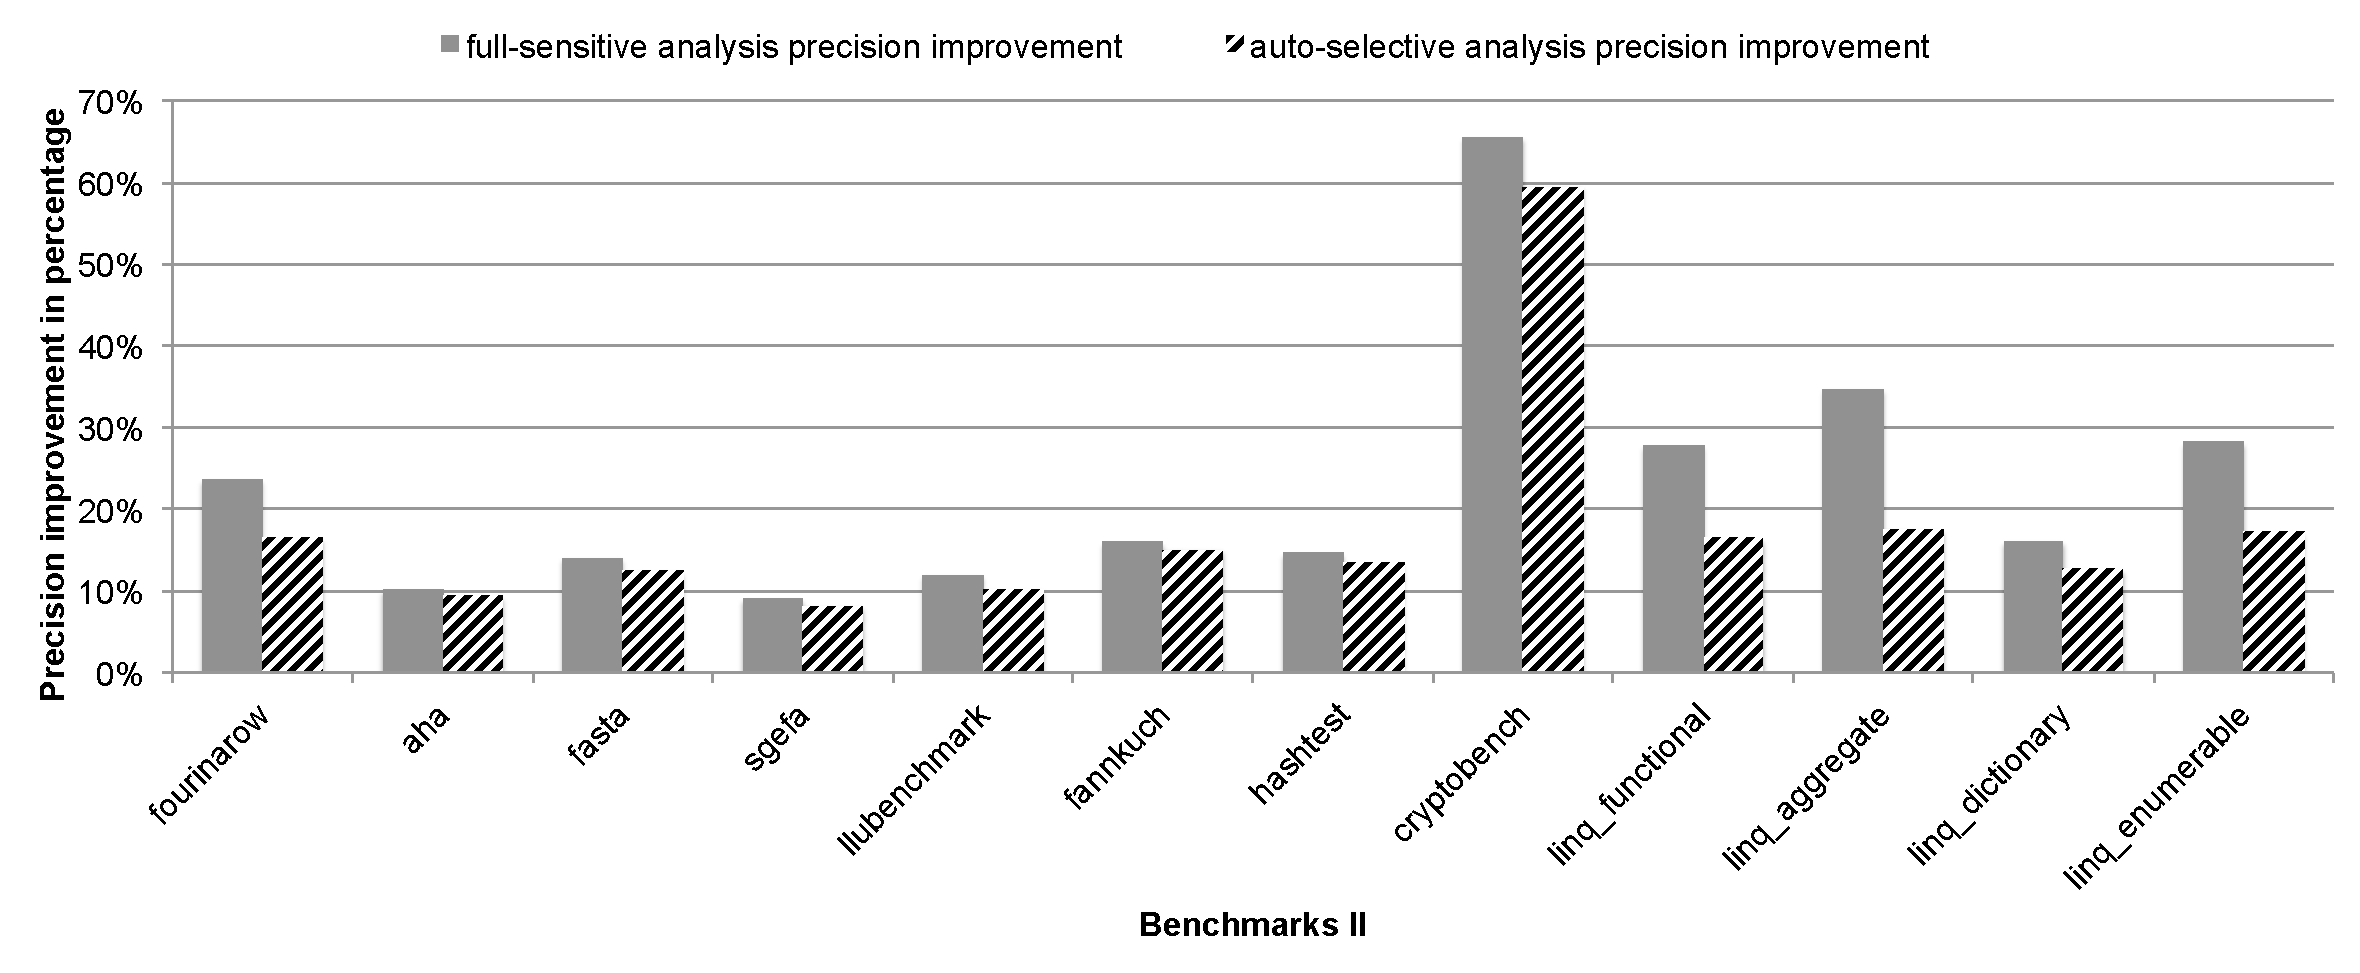
\includegraphics[width=2\columnwidth]{b2-precision}
\caption{\textmd{Benchmarks II precision results.}}
\vspace{-6pt}
\label{fig:b2-precision}
%\vspace{-6pt}
\end{figure*}

\begin{figure*}[th!]
        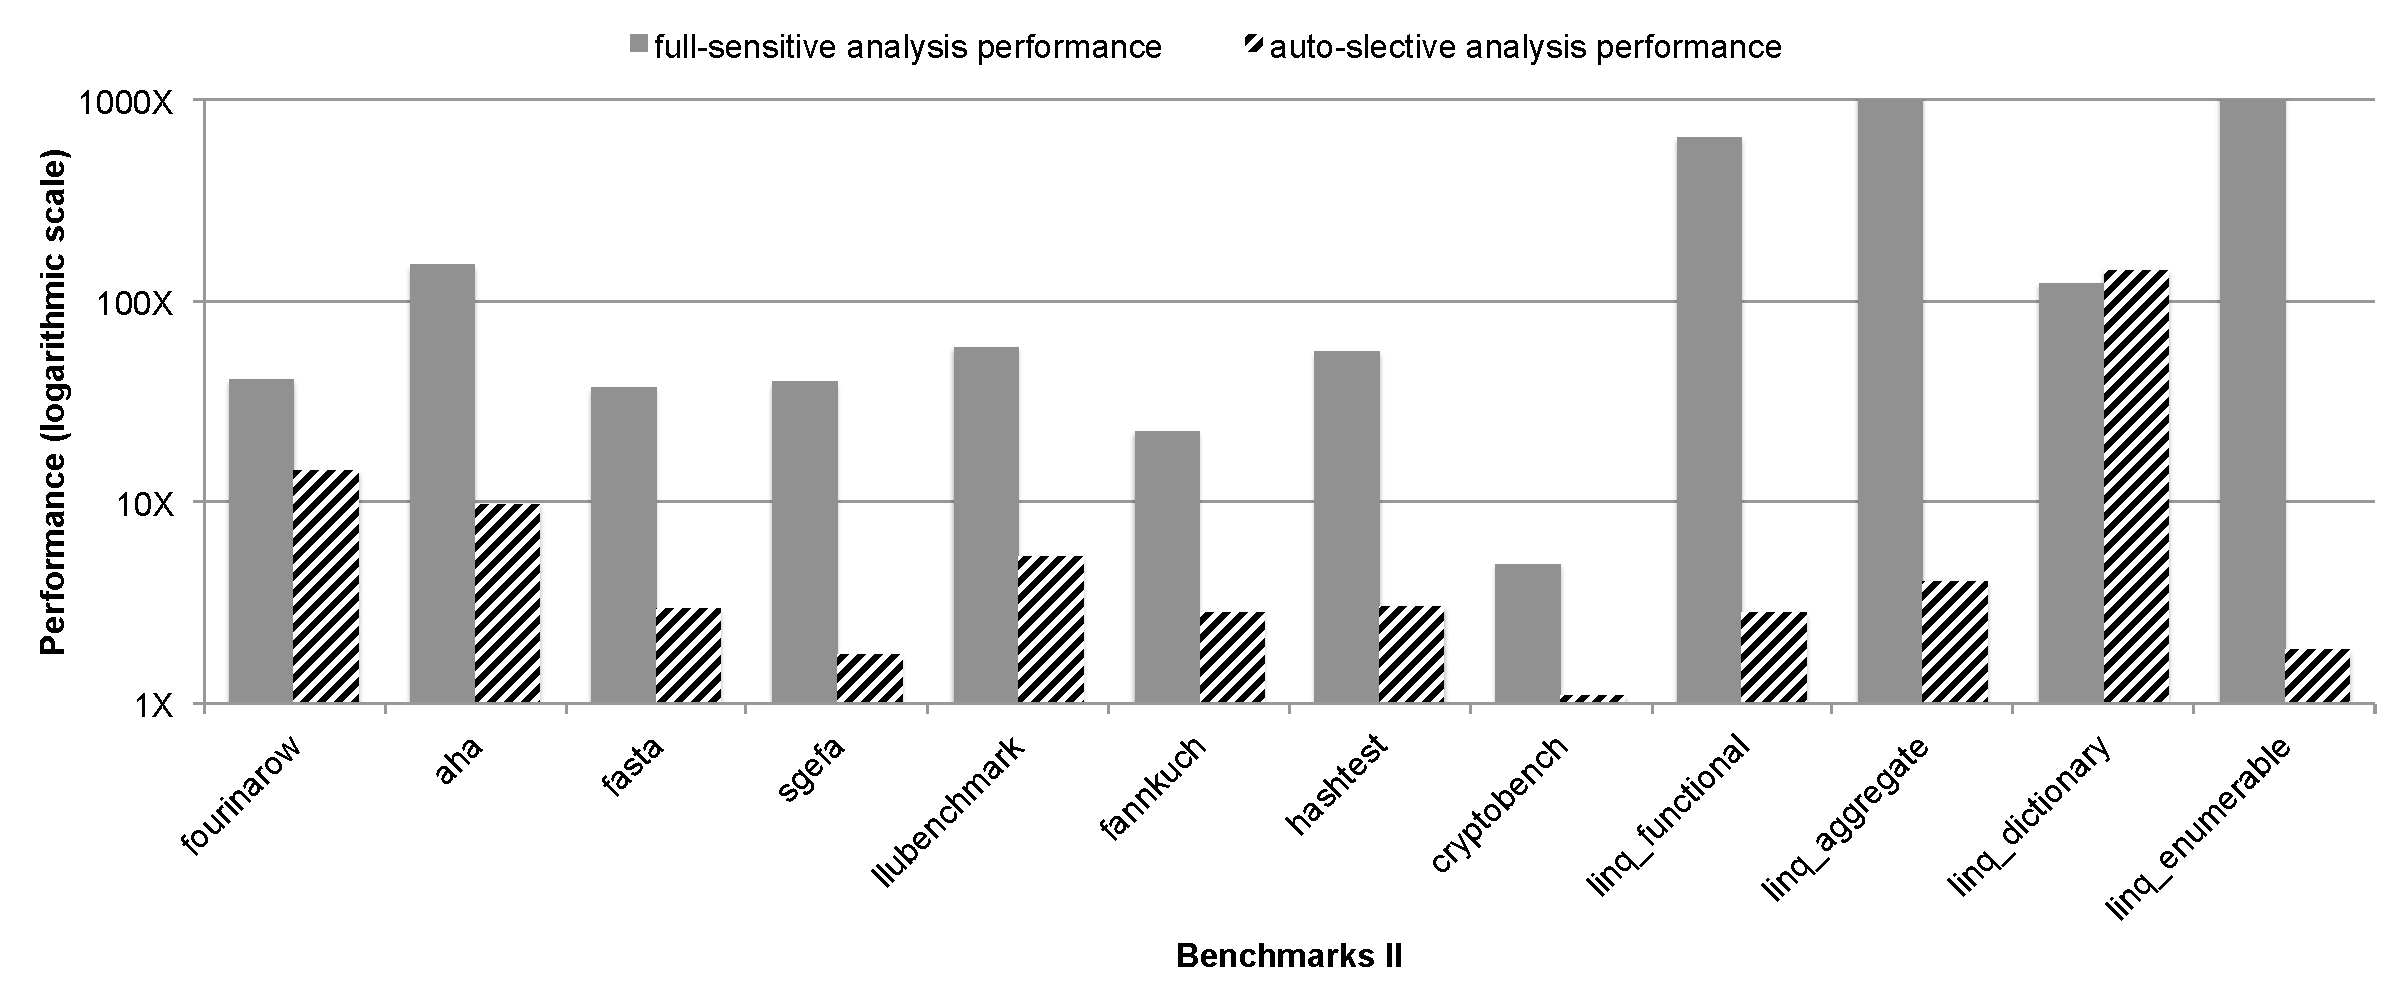
\includegraphics[width=2\columnwidth]{b2-performance}
\caption{\textmd{Benchmarks II performance results.}}
\vspace{-6pt}
\label{fig:b2-performance}
%\vspace{-6pt}
\end{figure*}

\subsection{Benchmarks II Results}
\label{b2-res}

{\bf TODO: the precision and performance results of the {\it auto-selective} results and discussions on the accuracy of improvement suggestion algorithm.}

Figures \ref{fig:b2-precision} and \ref{fig:b2-performance} show the precision and performance results of Benchmarks II, respectively. Because the {\it baseline} analysis finishes analyzing all 12 programs in Benchmarks II within the time budget of 10 minutes, the root cause localization was performed after the {\it baseline} points-to analysis completes on each program.

Figure \ref{fig:b2-precision} presents the {\tt PTS\_SIZE} precision improvement of the {\it straw man} (i.e., grey bars) and the {\it selective} (i.e., patterned bars) analyses over the {\it baseline} analysis. Because the {\it straw man} analysis applies 1-CFA and argument sensitivity over all the functions, its results are at least as precise as the {\it selective} analysis. In Figure \ref{fig:b2-precision}, the y axis shows the precision improvement of the corresponding analysis {\tt Y} over the {\it baseline} analysis {\tt BASE}, calculated as follows

\[
  {\tt IMP_{Y} = {{PTS\_SIZE_{BASE} - PTS\_SIZE_{Y}} \over {PTS\_SIZE_{BASE}}} \times 100\%}
\]

Therefore, {\tt IMP\textsubscript{Y}} measures analysis {\tt Y}'s precision in terms of removing the false positives from the {\it baseline} analysis results. In Figure \ref{fig:b2-precision}, the {\it straw man} analysis improves the {\tt PTS\_SIZE} precision by between 9\% (for {\it sgefa}) to 29\% (for {\it linq\_functional}). For all but three programs (i.e., {\it fourinarow}, {\it linq\_functional} and {\it linq\_aggregate}), the differences of the precision improvement percentages are within 3.2\% between the {\it straw man} and the {\it selective} analyses, indicating that the {\it selective} analysis produces similar results to the {\it straw man} analysis for most programs. The results of the {\it linq\_functional} program exhibit the largest difference in terms of precision improvement (i.e., 9.7\%) between the {\it straw man} (24.9\%) and the {\it selective} (15.2\%) analyses. Nevertheless, more than 60\% of the false positives that are produced by the {\it baseline} analysis, but not the {\it straw man} analysis, are absent from the {\it selective} analysis results for this program.

Figure \ref{fig:b2-performance} presents the performance results of the {\it straw man} (i.e., grey bars) and the {\it selective} (i.e., patterned bars) analyses comparing to the {\it baseline} analysis performance. The y axis shows the percentage of the corresponding analysis {\tt Y}'s time cost over the {\it baseline} analysis time (i.e., ${\tt \frac{TIME_{Y}}{TIME_{BASE}}}$). The performance of an analysis on each benchmark program was obtained by averaging over 30 repeated executions.

In Figure \ref{fig:b2-performance}, the {\it straw man} analysis performs worse than the {\it baseline} analysis for all the benchmark programs, for 4 programs (i.e., {\it fourinarow}, {\it aha}, {\it sgefa} and {\it llubenchmark}) about 100 times slower and another 5 programs ({\it frannkuch}, {\it hashtest}, {\it linq\_aggregate}, {\it linq\_dictionary} and {\it linq\_enumerable}) about an order of magnitude slower. For example, it takes less than one second for the {\it baseline} analysis to finish analyzing {\it fourinarow}, while the {\it straw man} analysis needs about 2 minutes to complete analyzing the same program. Despite of the fact that the {\it straw man} analysis often results in relatively significant precision improvement (e.g., 19.6\% for {\it fourinarow}), the performance issues outweigh the benefits of this whole-program combined context-sensitive analysis in many cases.

On the other hand, the {\it selective} analysis is capable of analyzing the benchmarks under the same order of magnitude as the {\it baseline} analysis for all but three programs (i.e., {\it fourinarow}, {\it cryptobench} and {\it linq\_dictionary}). For example, the {\it selective} analysis improves the precision over the {\it baseline} analysis by 21.7\% for {\it linq\_aggregate} and it also finishes analyzing this program more than 40\% faster than the {\it baseline} analysis. In most cases, the {\it selective} analysis results in a much better balance between performance and precision than the {\it straw man} analysis (e.g., the {\it straw man} analysis is 28.7\% more precise but performs about 7 times slower than the {\it baseline} analysis for {\it linq\_aggregate}). For three programs the {\it selective} analysis performs more than 10 times slower than the {\it baseline} analysis (i.e., 13, 14 and 17 times slower for {\it cryptobench}, {\it fourinarow} and {\it linq\_dictionary}, respectively), the {\it selective} analysis is still an order of magnitude faster than the {\it straw man} analysis for {\it fourinarow} and is similar to the {\it straw man} analysis in performance for {\it linq\_dictionary}. An outlier is the performance of the {\it selective} analysis for {\it cryptobench}, which is about 3 times slower than the {\it straw man} analysis, indicating the {\it selective} analysis may have applied context sensitivity on a set of functions that result in performance overhead without significant precision improvement for this particular program. Nevertheless, the {\it selective} analysis has achieved significantly better performance than the {\it straw man} analysis for most of the programs in Benchmarks II.

Our localization algorithm identifies between 6\% (for {\it fourinarow}) to 27\% (for {\it linq\_aggregate}) of the functions as the sources of precision loss, with an average of 13\% of the functions over all the programs in Benchmarks II, a relatively small fraction.

In summary, the {\it selective} analysis obtains similar precision results to the {\it straw man} analysis that improves the precision of the {\it baseline} analysis; moreover, the {\it selective} analysis' performance is significantly better than the whole-program combined context-sensitive {\it straw man} analysis. This result suggests that our localization algorithm can accurately identify the small fraction of functions that benefit from context sensitivity both in performance and precision for Benchmarks II, consistent with our observations in Section \ref{b1-res}.

\begin{comment}
setup: 1. localization results are obtained after the baseline analysis finishes.

precision: 1. selective analysis precision improvement close to straw man analysis;

performance: 1. selective analysis performance close to baseline analysis; 2. there are some outliers.

other: 1. the percentage of localized functions is small

{\bf Precision.}

Figures \ref{} and \ref{} show the precision results of the JavaScript benchmarks.

A figure for the precision results.

{\bf Performance.}

Figures \ref{} and \ref{} show the performance results of the JavaScript benchmarks. The time (in seconds) reported in this section are the average time calculated by running the analysis for the same application for 30 times.

A figure for the performance results.

(can pick a subset of these benchmarks to show results of 1cfa and 1cfa+parameter, the differences in terms of time and precision).
\end{comment}

\subsection{Case Study}
\label{case-study}

\subsection{Discussions}

\begin{comment}
\begin{table}[h!]
\centering
\begin{tabular}{ | C{1in} | C{0.6in} | C{0.6in} | C{0.6in} | }
\hline
 {\bf benchmark program} & {\bf 0-1-CFA} & {\bf 1-CFA} & {\bf Selective 1-CFA} \\
 \hline
 fourinarow & 9.0 & 25.9 & 9.1 \\
 \hline
 aha & 4.0 & 14.6 & 5.7 \\
 \hline
  fasta & 4.7 & 5.4 & 5.0 \\
 \hline
  ems-sgefa & 9.2 & 34.0 & 12.6 \\
 \hline
  llubenchmark & 6.9 & 13.3 & 9.4 \\
 \hline
  fannkuch & 6.1 & 17.9 & 8.8 \\
 \hline
  hashtest & 5.4 & 15.5 & 7.6 \\
 \hline
  cryptobench & 6.2 & 6.5 & 8.7 \\
 \hline
\end{tabular}
\vspace{6pt}
\caption{\textmd{Comparison of analysis performance in seconds.}}
\vspace{-6pt}
\label{table:performance1}
\end{table}

\begin{table*}[h!]
\centering
\begin{tabular}{ | C{0.9in} | C{0.8in} | C{0.8in} | C{0.8in} | C{0.8in} | C{0.8in} | C{0.8in} | }
\hline
 {\bf benchmark program} & {\bf 0-1-CFA} & {\bf 1-CFA} & {\bf Combined context-sensitive Analysis} & {\bf Selective 1-CFA} & {\bf Selective combined context-sensitive analysis} & {\bf Automatic selective combined context-sensitive analysis}\\
 \hline
 linq\_functional & 5.8 & 14.4 & 8.6 & 10.8 & 7.3 & 6.2 \\
 \hline
 linq\_aggregate & 4.1 & 17.0 & 11.5 & 5.0 & 3.3 & 3.5 \\
 \hline
  linq\_dictionary & 4.1 & 16.0 & 37.8 & 15.6 & 21.9 & 10.4 \\
 \hline
 linq\_enumerable & 3.3 & 84.4 & 45.1 & 2.7 & 2.0 & 2.1 \\
 \hline
  \end{tabular}
\vspace{6pt}
\caption{\textmd{Comparison of analysis performance in seconds.}}
\vspace{-6pt}
\label{table:performance2}
\end{table*}

\begin{table}[h!]
\centering
\begin{tabular}{ | C{1in} | C{0.6in} | C{0.6in} | C{0.6in} | }
\hline
 {\bf benchmark program} & {\bf 0-1-CFA} & {\bf 1-CFA} & {\bf Selective 1-CFA} \\
 \hline
 fourinarow & 6344 & 5296 & 5753 \\
 \hline
 aha & 3314 & 2996 & 3036 \\
 \hline
  fasta & 3066 & 2826 & 2858 \\
 \hline
  ems-sgefa & 4443 & 4207 & 4317 \\
 \hline
  llubenchmark & 3734 & 3308 & 3581 \\
 \hline
  fannkuch & 2540 & 2317 & 2377 \\
 \hline
  hashtest & 2798 & 2563 & 2660 \\
 \hline
  cryptobench & 8827 & 7624 & 7849 \\
 \hline
\end{tabular}
\vspace{6pt}
\caption{\textmd{Comparison of points-to analysis precision.}}
\vspace{-6pt}
\label{table:precision1}
\end{table}

\begin{table*}[h!]
\centering
\begin{tabular}{ | C{0.9in} | C{0.8in} | C{0.8in} | C{0.8in} | C{0.8in} | C{0.8in} | C{0.8in} | }
\hline
 {\bf benchmark program} & {\bf 0-1-CFA} & {\bf 1-CFA} & {\bf Combined context-sensitive Analysis} & {\bf Selective 1-CFA} & {\bf Selective combined context-sensitive analysis} & {\bf Automatic selective combined context-sensitive analysis}\\
 \hline
 linq\_functional & 2775 & 2144 & 2084 & 2707 & 2353 & 2354 \\
 \hline
 linq\_aggregate & 3036 & 2182 & 2166 & 2635 & 2376 & 2376 \\
 \hline
  linq\_dictionary & 2497 & 2231 & 2198 & 2324 & 2255 & 2255 \\
 \hline
   linq\_enumerable & 3380 & 3063 & 2702 & 3303 & 2813 & 2852 \\
 \hline
  \end{tabular}
\vspace{6pt}
\caption{\textmd{Comparison of points-to analysis precision.}}
\vspace{-6pt}
\label{table:precision2}
\end{table*}
\end{comment}